\documentclass[sisc-eikonal.tex]{subfiles}

\begin{document}

\begin{figure}
  \centering 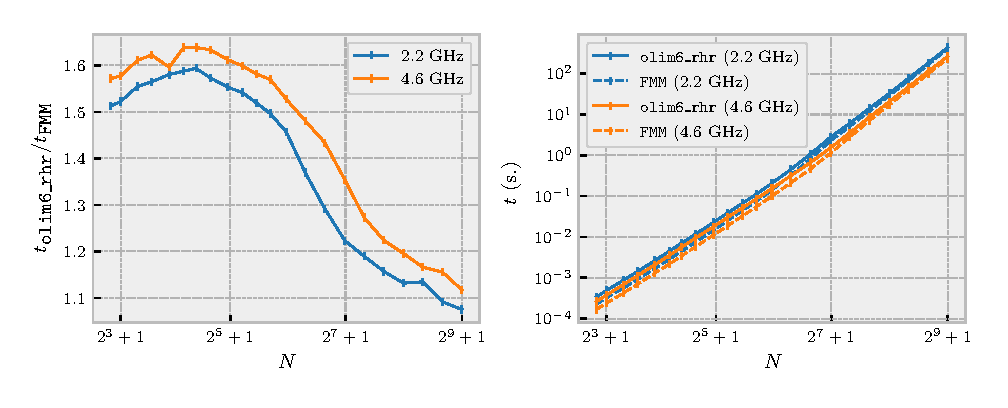
\includegraphics[width=\linewidth]{speed-comparison.eps}%
  \vspace{-1.5em}
  \caption{
    To see how much of a slowdown we get by using \texttt{olim6\_rhr}
    instead of the standard fast marching method (noting that they
    compute the same solution), we compare runtimes on two different
    computers. The first (labeled ``2.2 GHz'') is a 2015 MacBook Air
    with a 2.2 GHz Intel Core i7 CPU, 8 GB of 1600 MHz DDR3 RAM, a 256
    KiB L2 cache, and a 4 MiB L3 cache. The second (``4.6 GHz'') is a
    custom built workstation running Linux with a 4.6 GHz Intel Core
    i7 CPU, 64 GB of 2133 MHz DDR4 RAM, a 1536 KiB L2 cache, and 12
    MiB L3 cache. Both computers have L1 instruction caches and data
    caches that are each 32 KiB. From the plots, we can see that the
    difference in memory speeds has a significant impact on the
    relative slowdown. The plots here use our standard
    $\Omega = [-1, 1]^3$ domain $s \equiv 1$ and a point source at the
    origin, and discretized into $N = 2^p + 1$ nodes in each
    direction. From left to right, we plot: 1) the ratio of runtimes
    (slowdown factor) versus $N$, 2) the total CPU runtime of each solver.
  }\label{fig:speed-comparison}
\end{figure}

\begin{figure}
  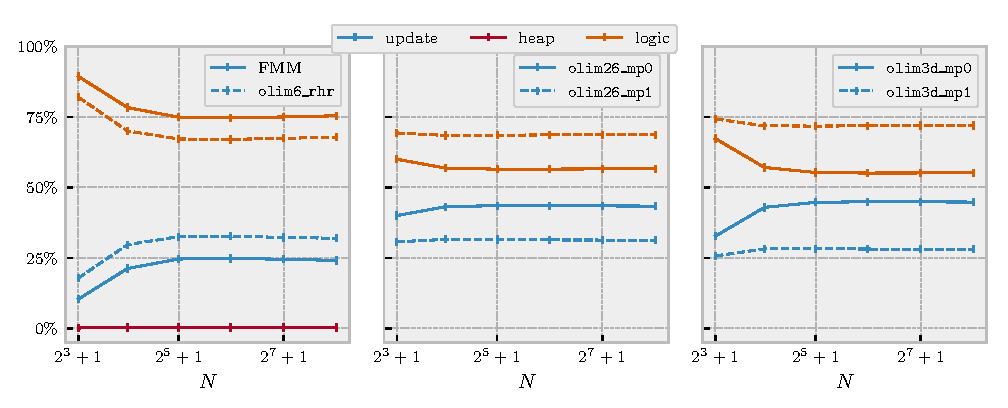
\includegraphics[width=\linewidth]{tasks.eps}%
  \vspace{-0.5em}
  \caption{ The percentage of time spent doing different tasks. The
    ``update'' tasks and ``heap'' tasks are clearly defined, while the
    ``logic'' task contains a variety of things related to
    control-flow, finding neighbors, and memory movement---basically,
    the parts of \cref{alg:dijkstra-like} that don't clearly pertain
    to computing new $\hat{U}$ values or keeping \texttt{front}
    updated. From these plots, it is clear that memory speed plays a
    large role in determining efficiency. To some extent, even though
    the more complicated update procedures are slower, their slowness
    is hidden somewhat by memory latency as problem sizes grow. For
    large $N$ and some solvers (the middle and right plots), ``heap''
    takes too little time, and is not picked up by the
    profiler.}\label{fig:tasks}
\end{figure}

\section{Numerical Results}\label{sec:numerical-results} In this
section, we collect our numerical tests. We first test our factored
method on several different slowness functions with available exact
solutions for point source data. We also test our method on a linear
speed function (reciprocal of slowness) which has been shown to be
amenable to local factoring. For each quadrature rule described in
\cref{ssec:quadrature} (\texttt{mp0}, \texttt{mp1}, or \texttt{rhr}),
we have two 2D algorithms, \texttt{olim4} and \texttt{olim8},
corresponding to 4- and 8-point stencils, respectively. Since there is
no advantage in 2D, we don't apply the top-down or bottom-up
approaches. In 3D, we have three top-down algorithms: \texttt{olim6}
(group IVa), \texttt{olim18} (groups I, IVa, and IVb), and
\texttt{olim26} (group V). We also test the bottom-up algorithm
\texttt{olim3d} (see \cref{fig:hu-neighborhoods}).

\subsection{Implementation Notes}\label{ssec:impl-notes}

Before describing our numerical tests, we briefly comment on our
implementation and make some observations about its
performance. Different design decisions can be made when implementing
a Dijkstra-like algorithm which significantly affect its performance
characteristics. We list the following choices that we made in our
implementation:
\begin{itemize}
\item We precompute and cache all values of $s$ on the grid $\calG$,
  as opposed to reevaluating $s$ each time a value is needed. We chose
  to do this because we assume that $s$ will generally be provided as
  gridded input data (consider, e.g., the shape from shading
  problem~\cite{kimmel2001optimal}, where the input data is an image).
\item We maintain the front using a priority queue implemented using
  an array-based heap, which is updated using the \texttt{sink} and
  \texttt{swim} functions described in Sedgewick and
  Wayne~\cite{sedgewick2011algorithms}.
\item The \texttt{front} data structure is stored as a dense grid of
  states: for each node in $p \in \calG$, we keep track of
  $p$\texttt{.state} for all time. Note that it is possible to
  maintain a sparse front which saves space but is slower to update.
\end{itemize}

We use a policy-based design~\cite{alexandrescu2001modern} written in
the C++ programmed language which makes heavy use of templates. This
allows us to conditionally compile different features and reuse logic
to implement different Dijkstra-like algorithms. In particular, we
implement the standard FMM~\cite{sethian1996fast} and make a direct
comparison between it and the ordered line integral method which it is
equivalent to, \texttt{olim6rhr} (see \cref{fig:speed-comparison}). We
have found that only a modest slowdown is incurred by using
\texttt{olim6rhr} for problems of moderate size. The disparity between
the two is greater for smaller problem sizes, which is due to cache
effects.

As a consequence of our design decisions, we note that our solvers
spend almost no time maintaing the front data structure. Using
Valgrind~\cite{nethercote2007valgrind}, we profiled running our solver
on the numerical tests below for different problem sizes and
categorized the resulting profile data. See \cref{fig:tasks}. The
``update'' task corresponds to time spent actually computing updates,
the ``logic'' task is a grab bag category for time spent on program
logic, and ``heap'' corresponds to updating the array-based heap which
implements \texttt{front}. Since the asymptotic complexity of the
``update'' and ``logic'' sections is $O(N^n)$, and since ``heap'' is
$O(N^n \log N)$, we can see from \cref{fig:tasks} that since so little
time is spent updating the heap, \emph{the algorithm's runtime is
  better thought of as $O(N^n)$ for practical problem sizes.}

\subsection[Single point source]{Slowness functions with an analytic
  solution for a point source}\label{ssec:point-source-problems}

Using \cref{eq:eikonal} directly, a simple recipe to create pairs of
slowness functions and solutions is to prescribe a continuous function
$u$ with level sets homeomorphic to balls, and compute
$s(x) = \norm{\nabla u(x)}_2$ analytically, which is valid for a
single point source at the origin. The motivation for this set of
tests is that it allows us to observe the effect of local factoring,
and allows us to see how \texttt{mp0}, \texttt{mp1}, and \texttt{rhr}
perform on different slowness functions. There is also a degree of
compensation between the accuracy obtained by improved directional
coverage (e.g., using \texttt{olim26} or \texttt{olim3d} instead of
\texttt{olim18}) and the error due to quadrature.

The following table shows our slowness function definitions:
\vspace{0.5em}
\begin{center}
  \begin{tabular}{cccc}
    Name & $u(x)$ & $s(x)$ \\
    \midrule
    \texttt{s1} & $\cos(r) + r - 1$ & $1 - \sin(r)$ \\
    \texttt{s2} & $r^2/2$ & $r$ \\
    \texttt{s3} & $S(x)^\top A S(x)$ & $\alpha\norm{\operatorname{diag}(C(x)){(A + A^\top)}S(x)}$ \\
    \texttt{s4} & $\tfrac{1}{2} x^\top A^{1/2} x$ & $\norm{x}_A = \sqrt{x^\top A x}$
  \end{tabular}
\end{center}
\vspace{0.5em} We assume that $x \in \Omega = [-1, 1]^3$. We also
define $r = \norm{x}$, and vector fields
$S(x) = (\sin(\alpha x_i))_{i=1}^3$ and
$C(x) = (\cos(\alpha x_i))_{i=1}^3$; we take $\alpha = \pi/5$. For
\texttt{s3} and \texttt{s4}, we assume that $A$ is symmetric positive
definite. In 3D, the matrices we use for \texttt{s3} and \texttt{s4}
are:\begin{equation} A_{\texttt{s3}} = \begin{bmatrix}
    1 & \nicefrac{1}{4} & \nicefrac{1}{8} \\
    \nicefrac{1}{4} & 1 & \nicefrac{1}{4} \\
    \nicefrac{1}{8} & \nicefrac{1}{4} & 1
  \end{bmatrix} = A_{\texttt{s4}}^{1/2}
\end{equation}

Our results are displayed in \cref{fig:time-vs-error}. We include
plots of relative $\ell_\infty$ error plotted versus problem size and
time. We summarize our observations:
\begin{itemize}
\item For all slowness functions, we can see that for \texttt{rhr}, as
  we increase directional coverage (\texttt{olim6\_rhr} $\to$
  \texttt{olim18\_rhr} $\to$ \texttt{olim26\_rhr}), our accuracy
  deteriotes---we should not lose the overall $O(h)$ convergence
  (although, see \cref{table:qv-least-squares} to see what happens to
  the convergance rate for the linear speed function), but the error
  constant becomes worse. On the other hand, using one of the midpoint
  rules allows improved directional coverage to translate into an
  improved error constant. Indeed, for all slowness functions and
  \texttt{mp0} or \texttt{mp1}, the error constants appear to be
  sorted by degree of directionality (\texttt{olim6} $<$
  \texttt{olim18} $<$ \texttt{olim26} $<$ \texttt{olim3d}). Although
  the exact range and deviation of error constants for the different
  slowness functions varies somewhat, the overall pattern remains the
  same. This phenomenon, surprising at first glance, is due to the
  fact that the contributions to the local error by \texttt{rhr} and
  the linear interpolation of $s$ partially compensate each other. The
  improvement of directional coverage reduces the interpolation error,
  and hence reduces the compensation of the error generated by
  \texttt{rhr} (see~\cite{yang2019computing} for a more detailed
  discussion).
\item If we scan each graph horizontally, we can see that the
  difference in error between \texttt{mp0} and \texttt{mp1} is
  difficult to discern. For each \texttt{mp1} graph, the corresponding
  \texttt{mp0} graph has the same error, but is shifted to the left,
  reflecting the fact that the \texttt{mp0} OLIMs are substantially
  faster. This fact is consistent with \cref{theorem:mp0-newton}, which
  justifies the use of \texttt{mp0}.
\item With respect to the choice of neighborhood, \texttt{olim6} is
  the fastest; and, for each choice of neighborhood, \texttt{mp0}
  provides the best combination of speed and accuracy. If we are
  willing to pay somewhat in speed, we can dramatically improve the
  error constant by improving the directional coverage and using a
  solver like \texttt{olim3d\_mp0}, which appears to be the best
  overall. This tradeoff is more pronounced for smaller problem
  sizes. A theme running through this work is that, as the problem
  size increases, memory access patterns come to dominate the runtime,
  and the disparity between the faster and slower neighborhoods
  becomes less pronounced. To see this, compare the start of each
  graph in the top-left of the plots, and their ends in the
  bottom-right. We can observe, e.g., that the maximum horizontal
  distance between starting points and ending points has decreased
  significantly, which confirms this observation.
\item One benefit of our high accuracy algorithms is that they allow
  us to obtain a better solution on rough mesh sizes in 3D. This is
  important since opportunities to refine the mesh (and decrease $h$,
  thereby improving the error) are limited for 3D problems. On our
  workstation, a typical large 2D problem on $\Omega = [-1, 1]^2$ with
  $\boundary = \set{0}$ was discretized by setting $N = 2^{14} +
  1$. In 3D, solving the point source problem with
  $\Omega = [-1, 1]^3$ and $\boundary = \set{0}$ for $N = 2^{9} + 1$
  required a similar amount of memory. In 2D, $h = 2^{-13}$; in 3D,
  $h = 2^{-8}$---a significant difference (32 times worse).
\end{itemize}

\begin{figure}
  \centering 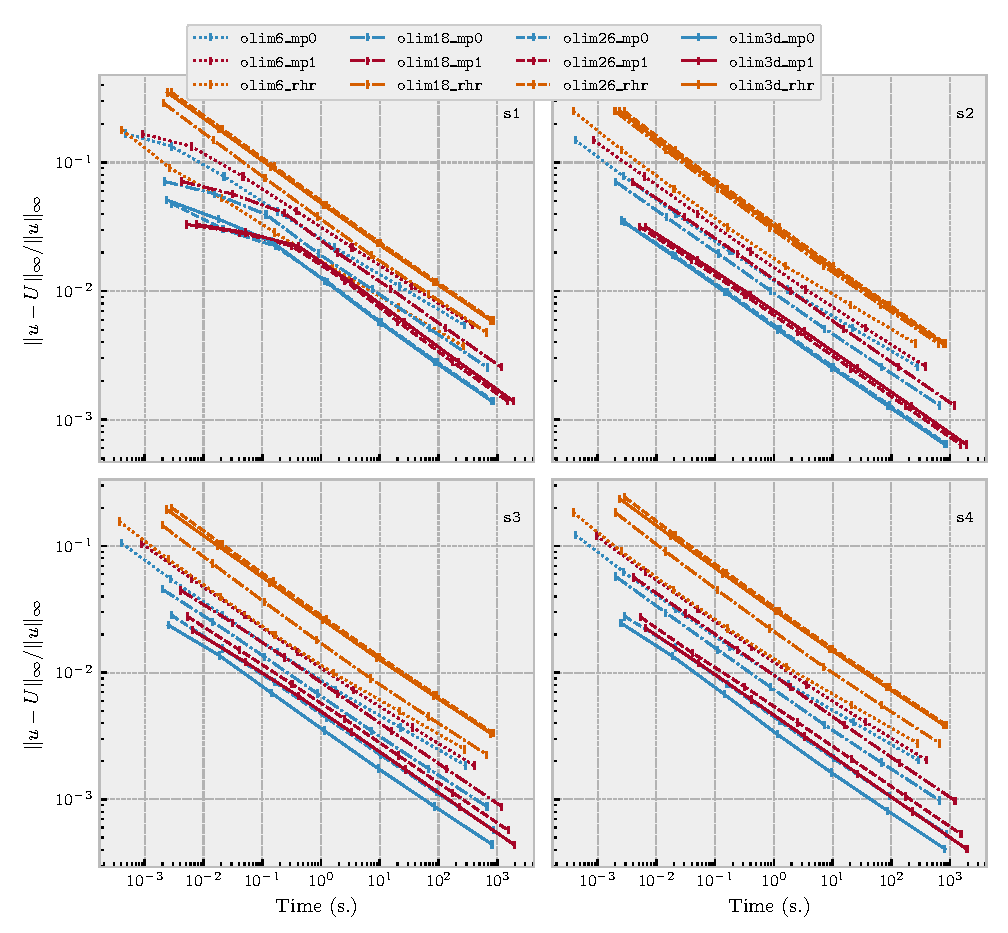
\includegraphics[width=\linewidth]{time_vs_error_3d.eps}
  \caption{Relative $\ell_\infty$ error plotted against CPU runtime in
    seconds. The domain is $\Omega = [-1, 1]^3$ discretized uniformly
    in each direction into $N = 2^p + 1$ points, where
    $p = 3, \hdots, 9$, so that there are $N^3$ points overall. The
    slowness functions used are listed in
    \cref{ssec:point-source-problems}. We note that the horizontal and
    vertical axes of each subplot are the
    same.}\label{fig:time-vs-error}
\end{figure}

\subsection{A linear speed function}\label{ssec:slotnick}

\begin{figure}
  \centering
  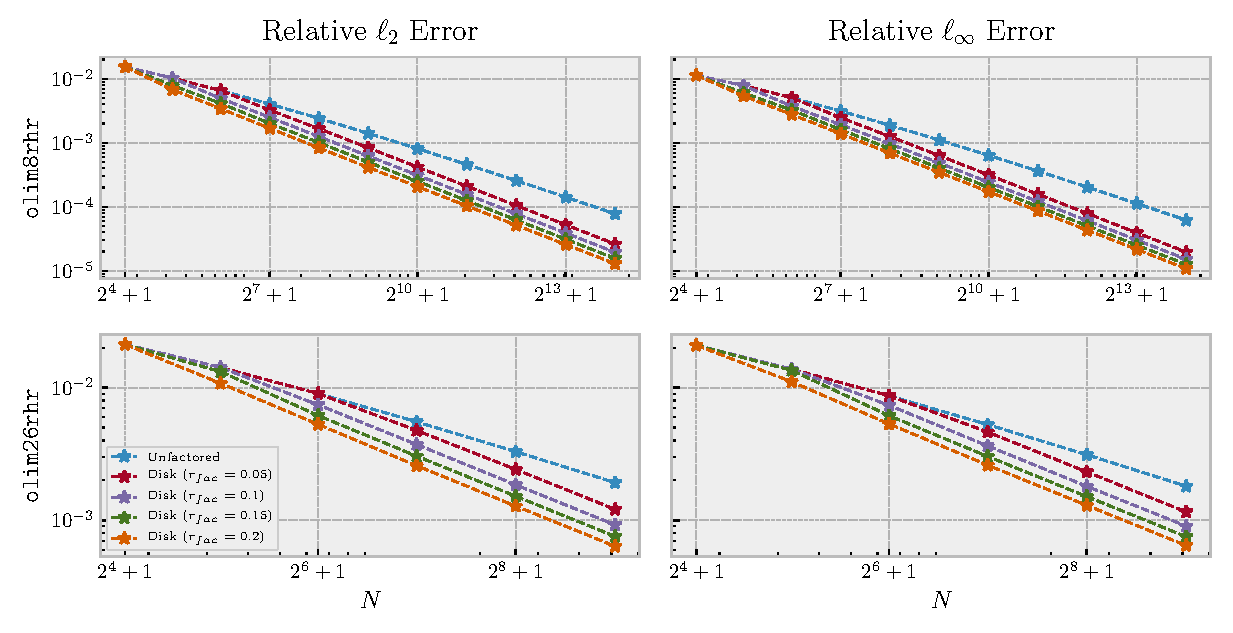
\includegraphics[width=\linewidth]{factoring-error-example.eps}%
  \vspace{-1.4em}
  \caption{Comparing different ways of selecting factored nodes. For
    the test problem, $\Omega = [-1, 1]^n$, with $n = 2$ (left) and
    $n = 3$ (right). The domain is descretized into $N^3$ nodes, where
    $N = 2^p + 1$, so that $h = 2/(N - 1)$. The slowness function is
    constant ($s \equiv 1$). For the 2D problem, \texttt{olim8rhr} is
    used; \texttt{olim26rhr} is used for the 3D problem. Solutions for
    the unfactored problem are plotted, along with solutions using a
    disk/sphere neighborhood with constant factoring radius given by
    $\rfac = 0.05, 0.1, 0.15, 0.2$. We note that for this problem the
    choice $\rfac = \sqrt{n}$ results in an exact solution. This only
    applies to the constant slowness function, $s \equiv 1$.
  }\label{fig:factoring-error-example}
\end{figure}

\begin{figure}
  \centering
  \vspace{-1em} 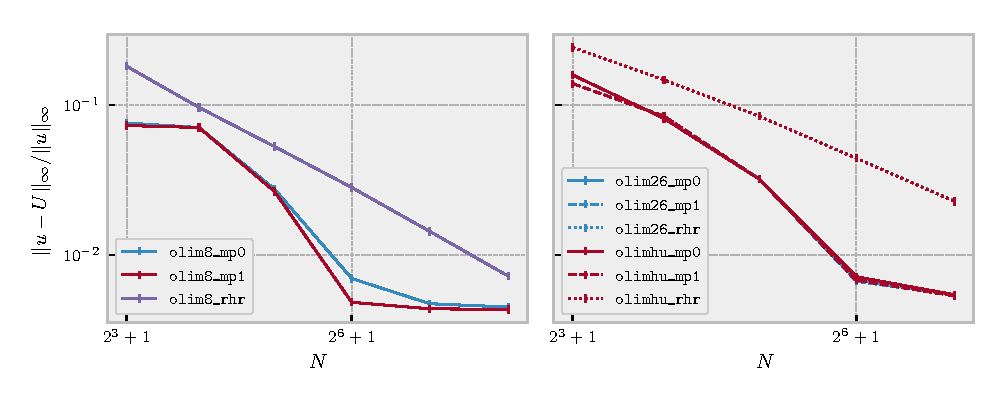
\includegraphics[width=\linewidth]{qv_plots.eps}%
  \vspace{-1.5em}
  \caption{Relative $\ell_\infty$ error plotted versus $N$ in 2D
    (left) and 3D (right).}\label{fig:qv}
  \vspace{-1em} 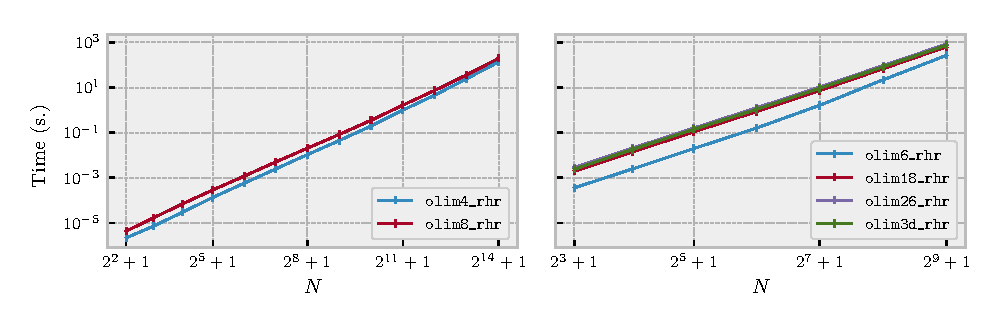
\includegraphics[width=\linewidth]{qv-time-plots.eps}%
  \vspace{-1.5em}
  \caption{Wall clock time plotted versus $N$ in 2D (left) and 3D
    (right).}\label{fig:qv-time-plots}
  \vspace{-1em}
  \caption*{Numerical results for \cref{ssec:slotnick}. Problem sizes
    are $N = 2^p + 1$, where $p = 3, \hdots, 14$ in 2D and
    $p = 3, \hdots, 9$ in 3D. The total number of nodes is $N^n$,
    where $n = 2, 3$. See \cref{ssec:slotnick} for least squares
    fits.}
\end{figure}

We consider a problem that has a known analytical solution and has
been used as a test problem for other factored eikonal equation
solvers before\footnote{We thank D.\ Qi for helpful discussions
  regarding this
  problem.}~\cite{slotnick1959lessons,fomel2009fast,qi2018corner}. For
a single point source at $x_i$ and a vector $v$, we define:
\begin{equation}
  \label{eq:slotnick-single-source}
  \frac{1}{s(x)} = \frac{1}{s(x_i)} + v^\top {(x - x_i)},,
\end{equation}
where $s_i = s(x_i)$. The analytic solution to \cref{eq:eikonal} for a
single source and slowness function given by
\cref{eq:slotnick-single-source} is~\cite{slotnick1959lessons}:
\begin{equation}
  \label{eq:slotnick-single-source-solution}
  u_i(x) = \frac{1}{\norm{v}} \cosh^{-1} \parens{1 + \frac{s_i}{2} s(x) \norm{v}^2 \norm{x - x_i}^2}.
\end{equation}
If we shift the point source from $x_i$ to another location $x_j$, we
find:
\begin{equation}
  \label{eq:slotnick-slowness-shift}
  \frac{1}{s_i} + v^\top {(x - x_j + x_j - x_i)} = \frac{1}{s_i} + v^\top {(x_j - x_i)} + v^\top {(x - x_j)} = \frac{1}{s_j} + v^\top {(x - x_j)}.
\end{equation}
That is, the slowness function $s$ remains unchanged as it is
rewritten with respect to a different source.

If $\set{x_i}$ is a set of point sources and $u_i$ is the solution of
the eikonal equation for the single point source problem with point
source given by $x_i$, then the solution for the multiple point source
problem with sources $\set{x_i}$ is:
\begin{equation}
  u(x) = \min_i u_i(x).
\end{equation}
We use this formula to compare relative $\ell_\infty$ errors for each
of our OLIMs in 2D and \texttt{olim26} and \texttt{olim3d} in 3D for
this slowness function with a pair of point sources, $x_1 = (0, 0)$
and $x_2 = (0.8, 0)$ in 2D, and $x_1 = (0, 0, 0)$ and
$x_2 = (0.8, 0, 0)$ in 3D. We set the domain of the problem to be
$\Omega = [0, 1]^n$ and discretize it into $N = 2^p + 1$ points, so
that $h = (N-1)^{-1}$.

For this choice of slowness function, we plot the CPU runtime versus
$N$ (see \cref{fig:qv-time-plots}), along with the relative
$\ell_\infty$ error versus $N$ (see \cref{fig:qv}). We also do least
squares fits for these plots to get an overall sense of the accuracy
and speed (see \cref{table:qv-least-squares}). Since we have
established that \texttt{olim8}, \texttt{olim26}, and \texttt{olim3d}
are the best choice of neighborhoods in the previous section, we do
not plot these results for \texttt{olim4}, \texttt{olim6}, and
\texttt{olim18}.

We can see that our conclusions from \cref{ssec:point-source-problems}
also hold for the multiple point source problem. Additionally, our
least-squares fits indicate to us that our algorithms' runtimes are
accurately described by the fit $T_N \sim C_T N^{\alpha}$ with
$\alpha \approx n$, and the error by $E_N \sim C_E h^{\beta}$, with
$\beta \approx 1$ (here, $E_N$ is the relative $\ell_\infty$
error). In fact, for \texttt{olim26} and \texttt{olim3d} with
\texttt{mp0} or \texttt{mp1}, the power $\beta$ is improved beyond $1$
to $\beta \approx 1.3$.

\begin{table}
  \begin{subtable}{0.5\textwidth}
    \centering
    {
      \small
      \begin{tabular}{ccc}
        Neighborhood & $C_T$ & $\alpha$ \\
        \hline \noalign{\vskip 0.2em}
        \texttt{olim4} & $7.779\times 10^{-8}$ & 1.0785 \\
        \texttt{olim8} & $1.971\times 10^{-7}$ & 1.0515 \\
        \hline \noalign{\vskip 0.2em}
        \texttt{olim6} & $2.968\times 10^{-7}$ & 1.085 \\
        \texttt{olim18} & $2.984\times 10^{-6}$ & 1.018 \\
        \texttt{olim26} & $4.649\times 10^{-6}$ & 1.0103 \\
        \texttt{olim3d} & $3.923\times 10^{-6}$ & 1.013 \\
      \end{tabular}
    }
    \caption{$T_N \sim C_T N^{\alpha n}$}
  \end{subtable}%
  \begin{subtable}{0.4999\textwidth}
    \centering
    {
      \small
      \begin{tabular}{ccc}
        Neighborhood & $C_E$ & $\beta$ \\
        \hline \noalign{\vskip 0.2em}
        \texttt{olim8\_mp0} & 0.4077 & 0.98744 \\
        \texttt{olim8\_mp1} & 0.3683 & 0.993 \\
        \texttt{olim8\_rhr} & 1.511 & 0.9728 \\
        \hline \noalign{\vskip 0.2em}
        \texttt{olim26\_mp0} & 2.328 & 1.3135 \\
        \texttt{olim26\_mp1} & 1.949 & 1.2888 \\
        \texttt{olim26\_rhr} & 1.772 & 0.90394 \\
        \hline \noalign{\vskip 0.2em}
        \texttt{olim3d\_mp0} & 2.268 & 1.3141 \\
        \texttt{olim3d\_mp1} & 1.865 & -1.2885 \\
        \texttt{olim3d\_rhr} & 1.77 & -0.90353
      \end{tabular}
    }
    \caption{$E_N \sim C_E h^\beta$}
  \end{subtable}
  \vspace{-1em}
  \caption{Least-squares fits of the runtime and relative
    $\ell_\infty$ error for OLIMs in 2D and 3D. We denote the time for
    a given $N$ by $T_N$; likewise, $E_N$ denotes the relative
    $\ell_\infty$ error for a specific $N$. We fit $T_N$ to a power
    $C_T N^\alpha$. In 2D, we expect $\alpha \approx 2$; in 3D,
    $\alpha \approx 3$. In 3D, we fit $E_N$ to $C_E h^\beta$, and
    expect $\beta \approx -1$ in all cases, due to the use of local
    factoring. In fact, for \texttt{olim26} and \texttt{olim3d} using
    either \texttt{mp0} or \texttt{mp1}, we find that the situation is
    better than expected, with
    $\beta \approx -1.3$.}\label{table:qv-least-squares}
\end{table}

\end{document}

%%% Local Variables:
%%% mode: latex
%%% TeX-master: "sisc-eikonal.tex"
%%% End:
